\documentclass[10pt,a4paper]{scrartcl}
\pagestyle{empty}
\usepackage{a4wide}
\usepackage[ngerman]{babel} % Neudeutsche Silbentrennung (mehrsprachiges Dokument)
\usepackage{parskip} % Skip indentation of first row
\usepackage{graphicx} % Graphics support
\usepackage{longtable} % Tables across several pages
\usepackage{booktabs}
\usepackage{mdwlist} % lists with less spacing, use itemize*
\usepackage{hyperref} % Hyperlinks
\usepackage{float} % Force float position
\usepackage[automark]{scrpage2} %kopf/fusszeile
\usepackage{listings}
\usepackage[utf8x]{inputenc} % Unicode-Encoding
\usepackage[framemethod=TikZ]{mdframed}
\usepackage{mdframed}
\usepackage{color}
\mdfdefinestyle{def}{%
	linecolor=gray!50!white,
	outerlinewidth=0.5pt,
	roundcorner=3pt,
	skipabove=\topskip,
	skipbelow=\topskip
	innertopmargin=\baselineskip,
	innerbottommargin=\baselineskip,
	innerrightmargin=10pt,
	innerleftmargin=10pt,
	nobreak=true
}

\definecolor{gray}{rgb}{0.4,0.4,0.4}
\definecolor{darkblue}{rgb}{0.0,0.0,0.6}
\definecolor{cyan}{rgb}{0.0,0.6,0.6}

\lstdefinelanguage{XML}
{
  morestring=[b]",
  morestring=[s]{>}{<},
  morecomment=[s]{<?}{?>},
  stringstyle=\color{black},
  identifierstyle=\color{darkblue},
  keywordstyle=\color{cyan},
  morekeywords={xmlns,version,type},% list your attributes here
  columns=fullflexible,
  showstringspaces=false,
  commentstyle=\color{gray}\upshape
}

\lstset{
	basicstyle=\linespread{.94}\ttfamily,
	tabsize=2,
}

\linespread{1.3}

\author{Danilo Bargen, Christian Fässler, Jonas Furrer} 
\title{strongTNC REST API\\SWID Measurement \\ \small{Im Rahmen der strongTNC BA} }

\pagestyle{scrheadings}
\ihead{REST API} %linke Kopfzeile
\ohead{strongTNC BA} %rechte Kopfzeile

\newcommand*{\escape}[1]{\texttt{\textbackslash#1}}

\let\textquotedbl="

\begin{document}

\begin{titlepage}
	\maketitle
	\vspace{120mm}
	\thispagestyle{empty} % Don't start page numbers on this page
\end{titlepage}

\newpage
	\tableofcontents
\newpage

\section{Ablauf der Messung}
Mittels POST auf die Ressource \texttt{http://tncserver/sessions/id/swid\_measurement} können Tags für eine Session gespeichert werden.
Hier der Auszug aus der REST API: \\
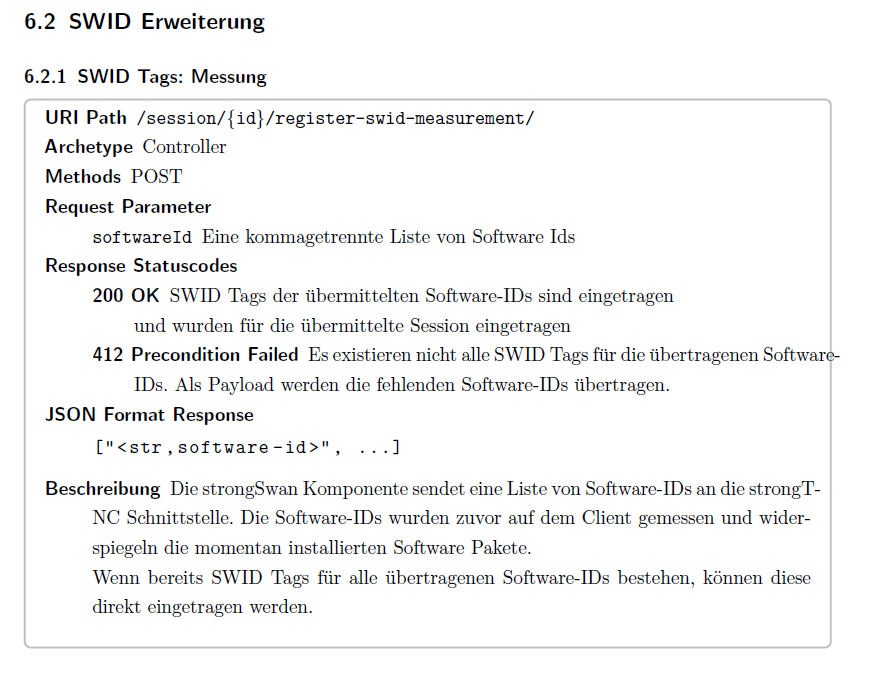
\includegraphics[scale=0.5]{swid-measurement-api.jpg}
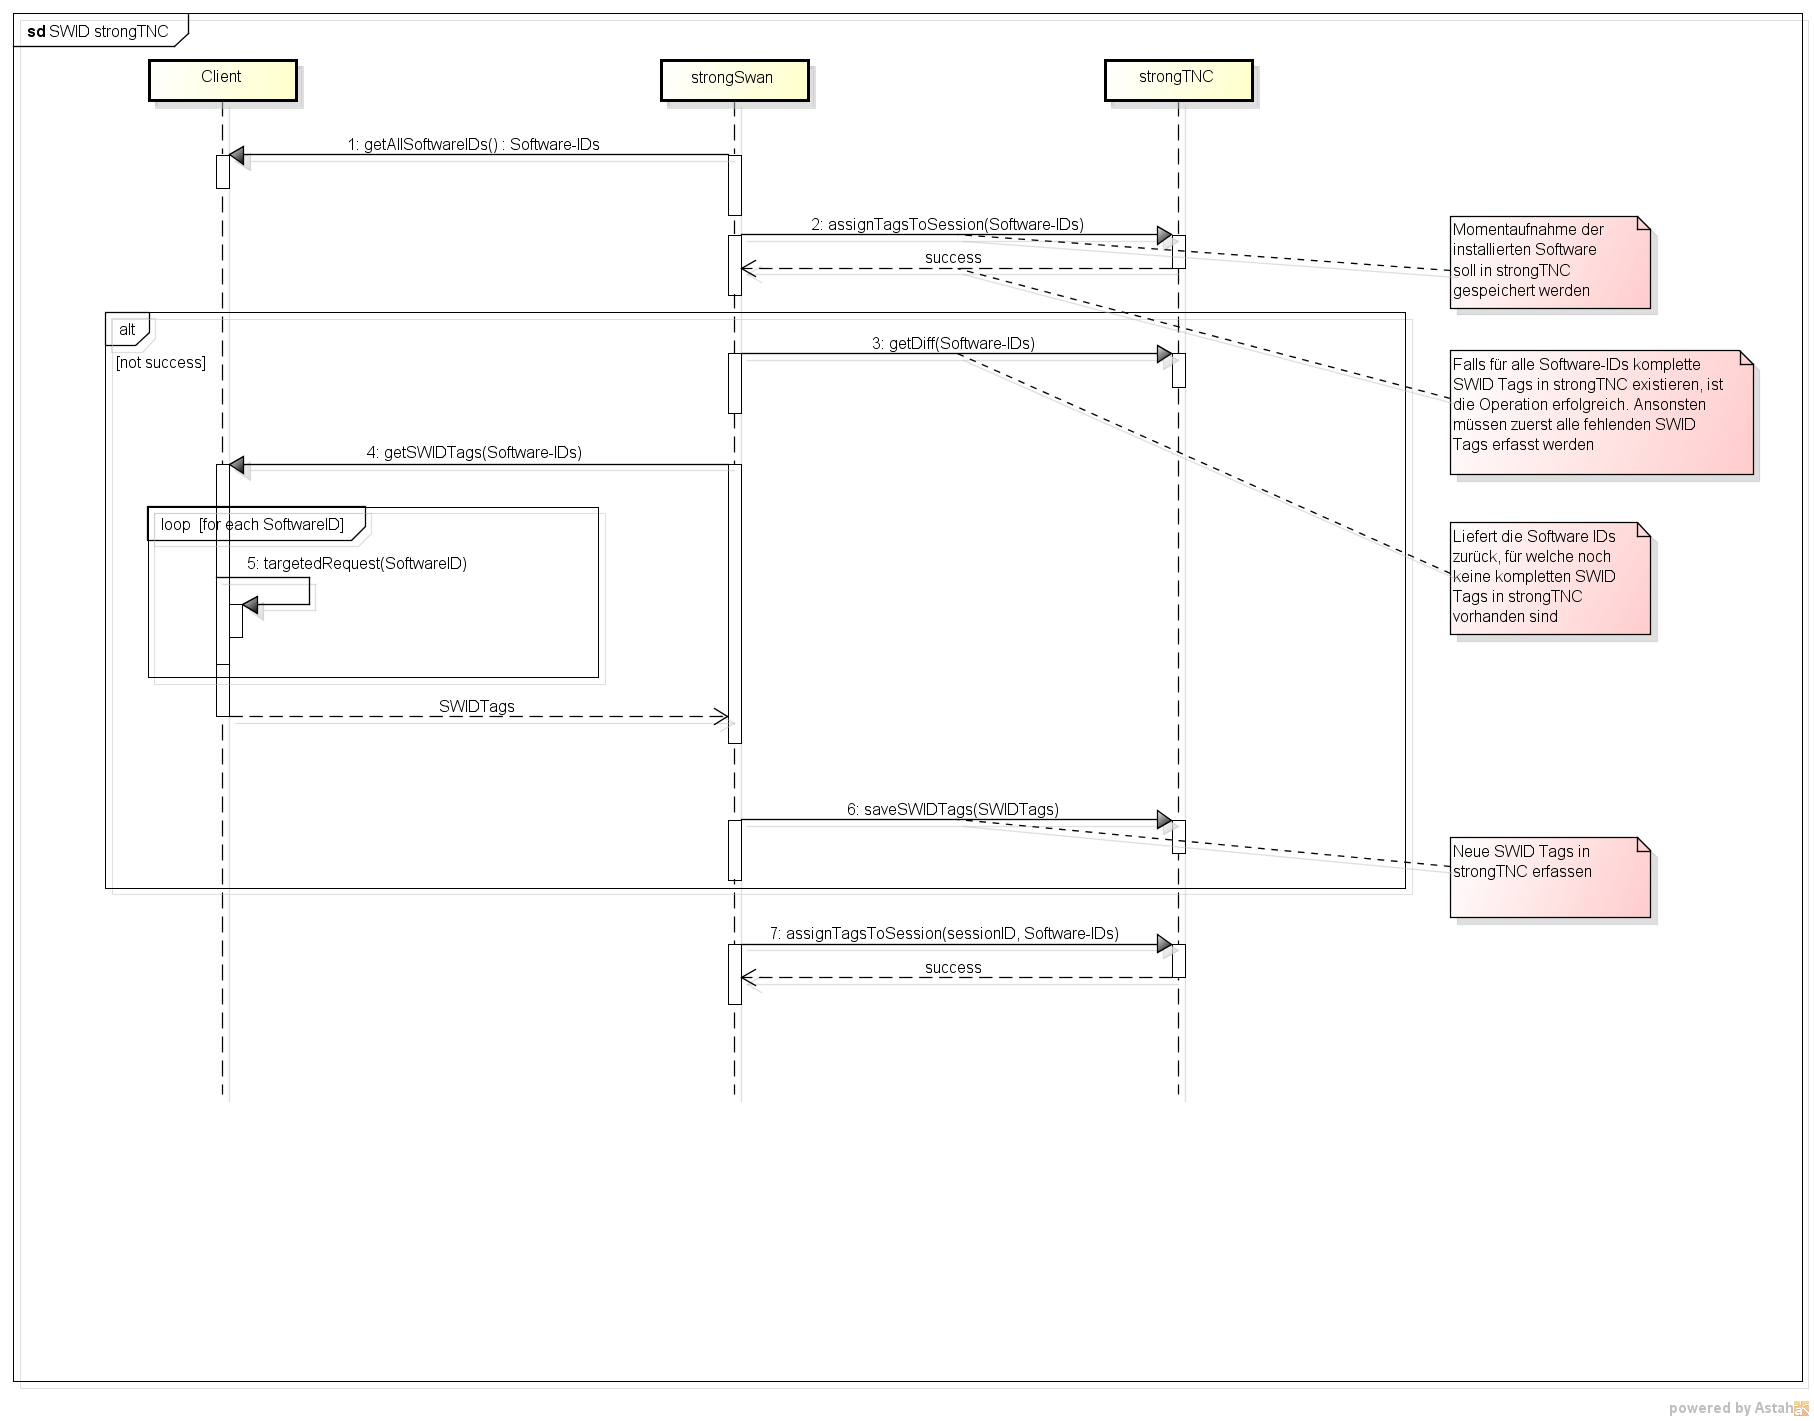
\includegraphics[scale=0.25]{../images/architecture/SWID_strongTNC.png}

\section{Beispiel Szenario}
Im folgenden soll der Ablauf einer Messung anhand eines konkreten Beispiels illustriert werden. In diesem Beispiel soll eine Messung für 3 Tags mit folgenden Software-IDs erfolgen:
\begin{itemize}
\item "regid.2004-03.org.strongswan\_Ubuntu\_12.04-i686-logrotate-3.7.8-6ubuntu5"
\item "regid.2004-03.org.strongswan\_Ubuntu\_12.04-i686-lsb-base-4.0-0ubuntu20"
\item "regid.2004-03.org.strongswan\_Ubuntu\_12.04-i686-strongswan-4.5.2-1.5+deb7u3"
\end{itemize}

\subsection{Request - SWID Measurement}
Als erstes wird versucht eine Messung für die Session mit der ID 2 zu erfassen. \hfill
\begin{lstlisting}

POST /api/sessions/2/swid_measurement/ HTTP/1.1
Authorization: Basic cm9vdDpyb290
User-Agent: curl/7.32.0
Host: tncserver:8000
Accept: */*
Content-Type: application/json
Content-Length: 239

[
"regid.2004-03.org.strongswan_Ubuntu_12.04-i686-logrotate-3.7.8-6ubuntu5",
"regid.2004-03.org.strongswan_Ubuntu_12.04-i686-lsb-base-4.0-0ubuntu20",
"regid.2004-03.org.strongswan_Ubuntu_12.04-i686-strongswan-4.5.2-1.5+deb7u3
]

\end{lstlisting}

Curl Befehl:
\begin{lstlisting}
curl	-i -X POST http://tncserver/sessions/2/swid\_measurement/ \
			-u root:root \
			-H "Content-Type: application/json" \
			-d $DATA
\end{lstlisting}
\subsubsection{Antwort - Status 412 Precondition Failed}
Sind noch nicht alle Tags in der strongTNC Datenbank vorhanden, werden dienigen Software-IDs zurückgeliefert, die zuerst erfasst werden müssen. Der HTTP Status Code ist 412 "Precondition Failed". Es werden zu diesem Zeitpunkt noch keine Tags mit der Session verknüpft. Eine entsprechende Antwort kann wie folgt aussehen:
\begin{lstlisting}
HTTP/1.0 412 PRECONDITION FAILED
Date: Wed, 14 May 2014 15:21:45 GMT
Server: WSGIServer/0.1 Python/2.7
Vary: Accept, Cookie
Content-Type: application/json
Allow: POST, OPTIONS

["regid.2004-03.org.strongswan_Ubuntu_12.04-i686-strongswan-4.5.2-1.5+deb7u3"]
\end{lstlisting}
\subsubsection{Antwort - Status 200 OK}
Wären für alle Software-IDs bereits Tags in der Datenbank vorhanden, könnte die Antwort wie folgt aussehen:
\begin{lstlisting}
HTTP/1.0 200 OK
Date: Wed, 14 May 2014 15:21:45 GMT
Server: WSGIServer/0.1 Python/2.7
Vary: Accept, Cookie
Content-Type: application/json
Allow: POST, OPTIONS

[]
\end{lstlisting}

\subsection{Nacherfassen von SWID Tags}
War die Messung nicht erfolgreich (Status 412), müssen für die zurückgelieferten Software-IDs zuerst komplette SWID Tags erfasst werden.
Im swidGenerator kann ein solcher mit \texttt{swid-generator swid --software-id="regid.2004-03.org.strongswan\_Ubuntu\_12.04-i686-fortune-mod-1:1.99.1-4"} abgefragt werden.
Ein solcher SWID Tag sieht wie folgt aus:

\lstset{language=XML}
\begin{lstlisting}
<?xml version="1.0" encoding="UTF-8"?>
<SoftwareIdentity name="strongswan" 
				  uniqueId="debian_7.4-x86_64-strongswan-4.5.2-1.5+deb7u3" 
				  version="4.5.2-1.5+deb7u3" versionScheme="alphanumeric" 
				  xmlns="http://standards.iso.org/iso/19770/-2/2014/schema.xsd">
  <Entity name="strongSwan" regid="regid.2004-03.org.strongswan" role="tagcreator"/>
  <Entity name="HSR" regid="regid.2004-03.org.strongswan" role="publisher"/>
  <Payload>
    <File location="/usr/share/doc/strongswan" name="README.gz"/>
    <File location="/usr/share/doc/strongswan" name="copyright"/>
    <File location="/usr/share/doc/strongswan" name="changelog.Debian.gz"/>
    <File location="/usr/share/doc/strongswan" name="CREDITS.gz"/>
    <File location="/usr/share/doc/strongswan" name="README.Debian.gz"/>
    <File location="/usr/share/doc/strongswan" name="NEWS.Debian.gz"/>
    <File location="/usr/share/doc/strongswan" name="changelog.gz"/>
  </Payload>
</SoftwareIdentity>

\end{lstlisting}

Dieser Tag kann anschliessend in der strongTNC Datenbank mittels POST Request auf die Ressource \texttt{/swid/add-tags/} erfasst werden. Die Daten für diesen Request bestehen aus einer JSON Liste von XML Strings, dadurch können auch mehrere Tags auf einmal erfasst werden. 
\paragraph{Tag Format}
\begin{itemize}
\item Die Dokumente können entweder mit oder ohne File Payload gespeichert werden. Wird versucht ein bereits bestehender Tag zu erfassen, wird dieser mit den neuen Daten komplett ersetzt.
\item XML Strings müssen in doppelten Anführungszeichen eingeschlossen und nichtdruckbare Zeichen innerhalb der XML Strings escapen werden (z.B newline, tab, double quotes $\rightarrow$ \escape{n}, \escape{t} \escape{"}).

\end{itemize}

Der Request sieht folgendermassen aus:
\lstset{
	basicstyle=\linespread{.94}\ttfamily,
	tabsize=2,
}
\begin{lstlisting}[language=BASH]

POST /api/swid/add-tags/ HTTP/1.1
Authorization: Basic cm9vdDpyb290
User-Agent: curl/7.32.0
Host: tncserver:8000
Accept: */*
Content-Type: application/json; charset="utf-8"
Content-Length: 239

[
"<?xml version=\"1.0\" encoding=\"utf-8\"?><SoftwareIdentity name=\"fortune-mod\"...",
"<?xml version=\"1.0\" encoding=\"UTF-8\"?><SoftwareIdentity name=\"strongswan\"..."
]
\end{lstlisting}

\end{document}

